\documentclass[a4paper,11pt,oneside]{report}

  \usepackage[T1]{fontenc}
  \usepackage[utf8]{inputenc}
  \usepackage{lmodern}

  \usepackage[a4paper]{geometry}
  \usepackage{titlesec}
  \usepackage{fancyhdr}
  \setlength{\headheight}{14.1595pt}

  \usepackage[hidelinks]{hyperref}
  \usepackage[tt]{titlepic}
  \usepackage{graphicx}
  \graphicspath{ {./images/} }

  \usepackage[spanish]{babel}

  \usepackage{float}
  \usepackage{picins}

  \usepackage{enumerate}

  \usepackage{pdfpages}

  %%%%%%%%%%%%%%%%%%%%%%%%%%%%%%%%%%%%%%%%%%%%%%%%%%%%%%%%%%%%%%%%%%%%%%%%%%%%%%%%
  % Paquete y definición de estilos para poder incluir código en el documento LaTeX
  % de manera formateada y con diseño
  %%%%%%%%%%%%%%%%%%%%%%%%%%%%%%%%%%%%%%%%%%%%%%%%%%%%%%%%%%%%%%%%%%%%%%%%%%%%%%%%

  \usepackage{listings}
  \usepackage{color}
  \definecolor{gray97}{gray}{.97}
  \definecolor{gray75}{gray}{.75}
  \definecolor{gray45}{gray}{.45}

  \lstset{ frame=Ltb,
    framerule=0pt,
    aboveskip=0.5cm,
    framextopmargin=3pt,
    framexbottommargin=3pt,
    framexleftmargin=0.4cm,
    framesep=0pt,
    rulesep=.4pt,
    backgroundcolor=\color{gray97},
    rulesepcolor=\color{black},
    %
    stringstyle=\small,
    showstringspaces = false,
    basicstyle=\tiny\small\ttfamily,
    commentstyle=\color{gray45},
    keywordstyle=\bfseries,
    %
    numbers=left,
    numbersep=15pt,
    numberstyle=\tiny,
    numberfirstline = false,
    breaklines=true,
    escapeinside=||,
  }
  \lstnewenvironment{listing}[1][]
  {\lstset{#1}\pagebreak[0]}{\pagebreak[0]}

  %%%%%%%%%%%%%%%%%%%%%%%%%%%%%%%%%%%%%%%%%%%%%%%%%%%%%%%%%%%%%%%%%%%%%%%%%%%%%%%%
  % Cabecera de los capítulos
  %%%%%%%%%%%%%%%%%%%%%%%%%%%%%%%%%%%%%%%%%%%%%%%%%%%%%%%%%%%%%%%%%%%%%%%%%%%%%%%%
  \makeatletter
    \def\@makechapterhead#1{%
      \hspace{0pt}%
      \vspace*{0\p@}%
      {\parindent \z@ \raggedright \normalfont
        \interlinepenalty\@M
        \Large\bfseries \thechapter.\quad #1\par\nobreak
        \vskip 10\p@
        \hrule
      }}
  \makeatother

  \makeatletter
    \def\@makeschapterhead#1{%
      \hspace{0pt}%
      \vspace*{0\p@}%
      {\parindent \z@ \raggedright \normalfont
        \interlinepenalty\@M
        \Large\bfseries #1\par\nobreak
        \vskip 10\p@
        \hrule
      }}
  \makeatother

  %%%%%%%%%%%%%%%%%%%%%%%%%%%%%%%%%%%%%%%%%%%%%%%%%%%%%%%%%%%%%%%%%%%%%%%%%%%%%%%%
  % Bibliografía como capítulo numerado
  %%%%%%%%%%%%%%%%%%%%%%%%%%%%%%%%%%%%%%%%%%%%%%%%%%%%%%%%%%%%%%%%%%%%%%%%%%%%%%%%

  \usepackage{etoolbox}
  \makeatletter
    \patchcmd{\thebibliography}{%
    \chapter*{\bibname}\@mkboth{\MakeUppercase\bibname}{\MakeUppercase\bibname}}{%
    \chapter{BIBLIOGRAFÍA}}{}{}
  \makeatother


  %%%%%%%%%%%%%%%%%%%%%%%%%%%%%%%%%%%%%%%%%%%%%%%%%%%%%%%%%%%%%%%%%%%%%%%%%%%%%%%%
  % Header superior derecha
  %%%%%%%%%%%%%%%%%%%%%%%%%%%%%%%%%%%%%%%%%%%%%%%%%%%%%%%%%%%%%%%%%%%%%%%%%%%%%%%%
  \pagestyle{fancyplain}
  \rhead{Miguel González Gómez}

  %%%%%%%%%%%%%%%%%%%%%%%%%%%%%%%%%%%%%%%%%%%%%%%%%%%%%%%%%%%%%%%%%%%%%%%%%%%%%%%%
  % 'dedication' environment: To add a dedication paragraph at the start of book %
  % Source: http://www.tug.org/pipermail/texhax/2010-June/015184.html %
  %%%%%%%%%%%%%%%%%%%%%%%%%%%%%%%%%%%%%%%%%%%%%%%%%%%%%%%%%%%%%%%%%%%%%%%%%%%%%%%%
  \newenvironment{dedication}
  {
     \thispagestyle{empty}
     \vspace*{\stretch{1}}
     \hfill\begin{minipage}[t]{0.66\textwidth}
     \raggedright
  }
  {
     \end{minipage}
     \vspace*{\stretch{3}}
  }

  %%%%%%%%%%%%%%%%%%%%%%%%%%%%%%%%%%%%%%%%%%%%%%%%%%%%%%%%%%%%%%%%%%%%%%%%%%%%%%%%
  % Enumeraciones de las secciones y subsecciones
  %%%%%%%%%%%%%%%%%%%%%%%%%%%%%%%%%%%%%%%%%%%%%%%%%%%%%%%%%%%%%%%%%%%%%%%%%%%%%%%%
  \renewcommand\thesection{\arabic{chapter}.\arabic{section}}
  \renewcommand\thesubsection{\thesection.\arabic{subsection}}

  %%%%%%%%%%%%%%%%%%%%%%%%%%%%%%%%%%%%%%%%%%%%%%%%%%%%%%%%%%%%%%%%%%%%%%%%%%%%%%%%
  % Interlileado
  %%%%%%%%%%%%%%%%%%%%%%%%%%%%%%%%%%%%%%%%%%%%%%%%%%%%%%%%%%%%%%%%%%%%%%%%%%%%%%%%
  \renewcommand{\baselinestretch}{1.2}

  %%%%%%%%%%%%%%%%%%%%%%%%%%%%%%%%%%%%%%%%%%%%%%%%%%%%%%%%%%%%%%%%%%%%%%%%%%%%%%%%
  % Se define la distancia entre párrafos como el doble de la distancia entre líneas
  %%%%%%%%%%%%%%%%%%%%%%%%%%%%%%%%%%%%%%%%%%%%%%%%%%%%%%%%%%%%%%%%%%%%%%%%%%%%%%%%
  \setlength{\parskip}{\baselineskip}

\begin{document}


%%%%%%%%%%%%%%%%%%%%%%%%%%%%%%%%%%%%%%%%%%%%%%%%%%%%%%%%%%%%%%%
% Generamos el título
%%%%%%%%%%%%%%%%%%%%%%%%%%%%%%%%%%%%%%%%%%%%%%%%%%%%%%%%%%%%%%%
% \title{\large \textbf {PROYECTO FINAL DE GRADO} \\ \ \\ \huge \textbf{Control inteligente del frigorífico en el hogar}}
% \author{Autor: Miguel González Gómez \and Director: Raúl García García}
% \date{19 de Marzo del 2014}
% \titlepic{\includegraphics[width=0.7\textwidth]{CEU_Universidad_San_Pablo.jpg}}

% \frontmatter
% \maketitle

\begin{titlepage}
\pagestyle{plain} %No headings for the first pages.
\begin{center}
        \Large
        \vspace{1cm}
        \bfseries\textbf{UNIVERSIDAD SAN PABLO - CEU\\}
        \vspace{1cm}
        \large
        \mdseries\textsf{ESCUELA POLITECNICA SUPERIOR\\}
        \vspace{0.5cm}
        \textsf{INGENIERÍA SUPERIOR EN TELECOMUNICACIONES\\
            E\\
            INGENIERÍA SUPERIOR EN INFORMÁTICA}
        \vspace{0.5cm}

        \begin{figure}[htbp]
            \centering
                \includegraphics[width=0.40\textwidth]{CEU_Universidad_San_Pablo.jpg}
            \label{fig:logoceu}
        \end{figure}

        \large
        \vspace*{2cm}
        \bfseries\textbf{PROYECTO FINAL DE GRADO\\}

        \Large
        \vspace*{1.5cm}
        \bfseries\textbf{Control inteligente del frigorífico en el hogar}
        \vspace{1cm}

        \large
        \bfseries\textbf{Autor: Miguel González Gómez\\
        Director: Raúl García García}
        \vspace{1.5cm}


        \mdseries\textsf{Junio 2014}
    \end{center}
\end{titlepage}


%%%%%%%%%%%%%%%%%%%%%%%%%%%%%%%%%%%%%%%%%%%%%%%%%%%%%%%%%%%%%%%
% Hoja de calificación
%%%%%%%%%%%%%%%%%%%%%%%%%%%%%%%%%%%%%%%%%%%%%%%%%%%%%%%%%%%%%%%

\includepdf[pages={1}]{pdf/calificacion.pdf}

%%%%%%%%%%%%%%%%%%%%%%%%%%%%%%%%%%%%%%%%%%%%%%%%%%%%%%%%%%%%%%%
% Dedicación
%%%%%%%%%%%%%%%%%%%%%%%%%%%%%%%%%%%%%%%%%%%%%%%%%%%%%%%%%%%%%%%
\begin{dedication}
Dedicated to my parents and sister \\
for their love, endless support \\
and encouragement.
\end{dedication}

%%%%%%%%%%%%%%%%%%%%%%%%%%%%%%%%%%%%%%%%%%%%%%%%%%%%%%%%%%%%%%%
% Agradecimientos
%%%%%%%%%%%%%%%%%%%%%%%%%%%%%%%%%%%%%%%%%%%%%%%%%%%%%%%%%%%%%%%

\chapter*{Agradecimientos} % si no queremos que añada la palabra "Capitulo"
\addcontentsline{toc}{chapter}{Agradecimientos} % si queremos que aparezca en el índice
\markboth{AGRADECIMIENTOS}{AGRADECIMIENTOS} % encabezado

Quisiera agradecer en primer lugar a mis padres y a mi hermana Beatriz. Gracias por haberme animado desde pequeño a perseguir aquello que más me gustara, por vuestro apoyo constante y por soportar todas aquellas horas que he pasado encerrado trasteando con el ordenador.

A mis compañeros de curso por la ayuda que me han brindado a lo largo de cuatro años, así como los buenos momentos que hemos pasado y seguiremos pasando. En especial a Jaime, Felipe, Javier y Yahi por los findes de semana que hemos estado encerrados estudiando en Villalba, fines de los que tengo grandes recuerdos. También, a Jorge, con quien he descubierto nuevas tecnologías, he asistido al evento Codemotion Madrid donde aprendimos un montón y en especial, por sus ánimos cuando he encontrado dificultades a la hora de realizar este proyecto.

Agradecer a mis compañeros de piso; Diane, Lydia, Raúl y Rubén, por aguantarme en el último año con el estrés de los trabajos y exámenes finales, y en especial, por soportar mis desorden debido a este proyecto. También, daros las gracias por haberme hecho disfrutar de los momentos libres que he tenido, así como de las vacaciones de navidad y verano.

A mis amigos de Logroño, quienes me han dado siempre su confianza a la hora de afrontar esta aventura. Y en especial, a mi amigo Álvaro por haber aguantado todas mis conversaciones sobre la carrera y los trabajos que he tenido que realizar.

Por último, me gustaría agradecer a la fundación Ramón Areces (El Corte Inglés) y su sistema de becas, así como a la Universidad CEU San Pablo, por darme la oportunidad de realizar este Grado en Ing. de Sistemas de Información y obtener una formación en un puesto de trabajo en el grupo de Informática El Corte Inglés, en concreto en Telecor, donde he podido formarme y crear amistades que no se van a olvidar.

%%%%%%%%%%%%%%%%%%%%%%%%%%%%%%%%%%%%%%%%%%%%%%%%%%%%%%%%%%%%%%%
% Abstracto
%%%%%%%%%%%%%%%%%%%%%%%%%%%%%%%%%%%%%%%%%%%%%%%%%%%%%%%%%%%%%%%

% Abstracto en español
\chapter*{Resumen}

El objetivo del proyecto es resolver un problema muy común en el hogar, el control de los gastos a la hora de llenar el frigorífico debido a una mala gestión de las compras. Además, se obtienen otros beneficios como; control de una dieta sana y equilibrada, evitar el desperdicio de alimentos que no se consumen, listas automáticas de los productos a comprar, estadísticas en tiempo real, etc.

Esta solución se divide en tres bloques principales:

 \begin{description}
    \item Componente electrónico

    Es la parte del proyecto más física donde se deberá ensamblar un aparato que permita la lectura de productos.

    Para ello se contará con dos tipos de entrada de productos; a través del código de barras ó un lector RFID, y de una salida Wireless para comunicar al servidor la entrada de los productos.

    \item Servidor centralizado

    Es la parte lógica del proyecto, el encargado de recibir la información del componente electrónico, almacenarla y operar con ella para ofrecer a las aplicaciones cliente acceso a toda la información.

    \item Aplicación cliente

    Es la parte de comunicación donde toda la información es consumida por el usuario a través de gráficas, resúmenes, listados, etc.

    Mediante el cruce de datos generado por el componente electrónico y toda la información contenida en el servidor se le mostrará al cliente la siguiente información:
        \begin{itemize}
        \item Stock actual del frigorífico
        \item Estadísticas de consumo; listados y estadísticas con los productos que se han comprado mediante el uso de filtros como; tipo de productos, fechas, precios...
        \item Estadísticas de gastos
        \end{itemize}

    Al emplear un servidor centralizado se va a permitir la creación de herramientas de colaboración entre los usuarios de la aplicación para la administración y creación de:
        \begin{itemize}
        \item Identificación de productos; nombre, precio, imagen, etc.
        \item Planes de compra; permitirá compartir planes de compra que pueden orientarse a distintos fines como el conseguir un ahorro económico.
        \item Recetas; de esta manera se podrá consultar en base al stock que se dispone en el frigorífico que recetas de cocina se pueden preparar.
        \end{itemize}
\end{description}

% Abstracto en inglés
\chapter*{Abstract}

Companies like LG have introduced smart fridges in the last years; fridges that can be controlled via smartphone and allow know the information about the products what contains inside thanks to smart labels.

The project aims to bring some of this technology to the user without having to make a large investment. No need to change the fridge, it has been built thanks to a \emph{Arduino component}, which allows scanner the products.

There are applications that allow control the spending at home, but unlike this project, they are focused to include the total cost of a purchase. This project allows you to scan product by product, and thanks to a collaborative data base, obtain the total cost of the purchase; distinguished by type of food... Also eating habits, create a shopping list, etc.

This solution was divided into three main blocks:

 \begin{description}
    \item Electronic Component

        It is part of the more physical project which has created a device that allows reading the products.

        To do this it has two input modes; through barcode or an RFID tag, and a wireless output to communicate to the server.

    \item Centralized Server

        It is the logic of the project, responsible for receiving the data from the electronic component, store it and server it to client applications.

    \item Client Application

            It is the communication part where all the information is consumed by the user through graphical summaries, lists, etc.

            By crossing data generated by the electronic component and all information contained on the server will show to the customer the following information:
            \begin{itemize}
                \item Current Stock of the fridge
                \item Consumption statistics; lists and statistics with the products purchased using filters like; product, dates, prices...
                \item Expenditure statistics
            \end{itemize}

            By using a centralized server will allow the creation of tools for collaboration between users of the application for the creation and management:

            \begin{itemize}
                \item Product identification; name, price, image, etc.
                \item Purchase plans; allow share purchase plans that can be adjusted to achieve different purposes like saving money.
                \item Recipes; this way you can see based on the stock that you have in the fridge which recipes can be prepared.
            \end{itemize}
\end{description}

%%%%%%%%%%%%%%%%%%%%%%%%%%%%%%%%%%%%%%%%%%%%%%%%%%%%%%%%%%%%%%%
% Índice autogenerado
%%%%%%%%%%%%%%%%%%%%%%%%%%%%%%%%%%%%%%%%%%%%%%%%%%%%%%%%%%%%%%%

\tableofcontents

%%%%%%%%%%%%%%%%%%%%%%%%%%%%%%%%%%%%%%%%%%%%%%%%%%%%%%%%%%%%%%%
% Índice de figuras
%%%%%%%%%%%%%%%%%%%%%%%%%%%%%%%%%%%%%%%%%%%%%%%%%%%%%%%%%%%%%%%

\cleardoublepage
\addcontentsline{toc}{chapter}{LISTA DE FIGURAS} % para que aparezca en el indice de contenidos
\listoffigures

%%%%%%%%%%%%%%%%%%%%%%%%%%%%%%%%%%%%%%%%%%%%%%%%%%%%%%%%%%%%%%%
% Capítulos
%%%%%%%%%%%%%%%%%%%%%%%%%%%%%%%%%%%%%%%%%%%%%%%%%%%%%%%%%%%%%%%

\input{introduccion/fribone-introduccion}

\chapter{ESTADO DE LA CUESTIÓN}

Estado

\section{DOMÓTICA}
\subsection{Sub Sección}
\section{ARDUINO}
\subsection{Introducción}
\subsection{Proyectos}
\section{CONCLUSIONES}

\chapter{REQUISITOS DEL SISTEMA}

Requisitos

\chapter{ARQUITECTURA DEL SISTEMA}

\section{Diagrama general}

Siguiendo los requisitos anteriormente explicados, se desarrolla un sistema basado en tres partes: componente hardware, servidor y aplicación cliente.

El diagrama general del sistema es el que se muestra en la siguiente figura:

\begin{figure}[H]
    \centering
    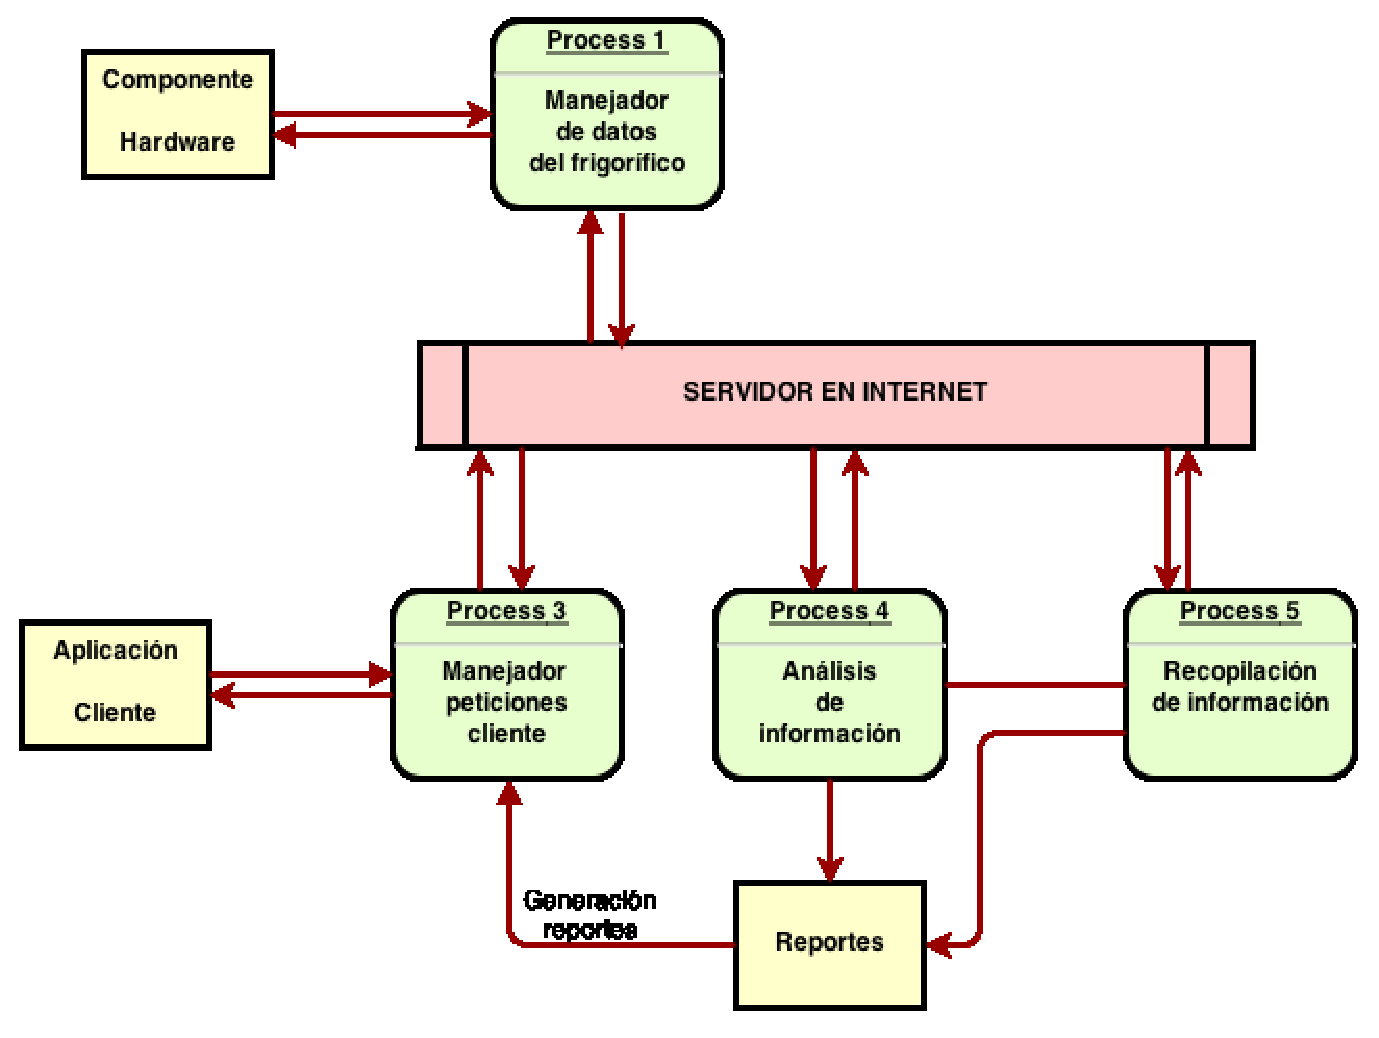
\includegraphics[keepaspectratio,width=0.9\textwidth]{diagrama-general.eps}
    \label{fig:diagrama-general}
\end{figure}

\chapter{DISEÑO E IMPLEMENTACIÓN}

Diseño e implementación

\chapter{CONCLUSIONES}

Este proyecto ha abordado el diseño y la construcción de un componente hardware apoyado por una plataforma en la nube para el seguimiento del consumo en el hogar, en concreto las compras realizadas en los supermercados. Para ello, se ha utilizado \emph{Arduino Yún} y una serie de componentes en el diseño del prototipo y de distintas tecnologías web para la construcción de la aplicación web.

La elección de este proyecto surgió de la curiosidad acerca de \emph{Arduino}, del creciente entusiasmo en cuantificar todo lo que se pueda y de la multitud de aplicaciones que se utilizan para llevar el control de los gastos en el hogar.

\section{Primer paso}

El primer paso en el proyecto fue hacerse con un \emph{Arduino} para empezar a jugar con él y familiarizarse con su entorno de programación. Simultáneamente se adquirió un lector de código de barras con conector \emph{USB HID}.

La versión de \emph{Arduino} elegida fue la \emph{UNO} debido a que su precio económico y a la amplia documentación que hay sobre la placa. El primer problema que se tuvo fue la falta de conexión \emph{USB} de la placa, se resolvió adquiriendo una \emph{Shield USB}. El segundo problema vino por la falta de conexión \emph{WiFi}, se intentó resolver adquiriendo una \emph{Shield WiFi} no oficial, pero no se logró hacer que funcionara.

Con estos problemas el segundo paso consistió en investigar y en conocer \emph{Arduino Yún}, una placa \emph{Arduino} que resuelve estos problemas ya que dispone de un puerto \emph{USB} y de un microprocesador con \emph{Linux} y conexión \emph{WiFi}. Con todos los componentes adecuados se diseñó el primer software para el escaneo de códigos de barras, el cual se guardaba a través de \emph{Internet} en un servidor.

\section{Segundo paso}

El segundo paso consistió en desarrollar la aplicación servidor utilizando para ello algunas de las piezas que componen las metodologías ágiles; control de versiones, tests unitarios e integración contínua.

\begin{itemize}

    \item Para el control de versiones se ha utilizado \emph{GitHub}, una plataforma que permite la creación de repositorios públicos de manera gratuita y que actualmente es la que más auge tiene en los proyectos de código abierto.

    \item Para los tests unitarios se ha utilizado \emph{PHPUnit} debido a que es uno de los frameworks más conocidos. Se tuvieron que resolver problemas con \emph{CodeIgniter} ya que no está pensado para realizar tests sobre él.

    \item Para la integración contínua se ha utilizado \emph{TravisCI}, una herramienta web que se sincroniza con tu cuenta de \emph{GitHub} para construir y pasar los tests unitarios de todas las modificaciones que realices sobre el repositorio.

\end{itemize}

\section{Tercer paso}

A continuación, con las primeras versiones de la aplicación servidor, se fue realizando el diseño de la página web utilizando para ello \emph{Bootstrap} y algunas librerías \emph{JavaScript} como; \emph{JQuery}, \emph{Director}, \emph{Handlebars}, etc.

\section{Cuarto paso}




\chapter{LÍNEAS FUTURAS}

Líneas futuras

%%%%%%%%%%%%%%%%%%%%%%%%%%%%%%%%%%%%%%%%%%%%%%%%%%%%%%%%%%%%%%%
% Bibliografía
%%%%%%%%%%%%%%%%%%%%%%%%%%%%%%%%%%%%%%%%%%%%%%%%%%%%%%%%%%%%%%%



\nocite{*}
\bibliographystyle{plain}
\bibliography{bibliografia/fribone-bibliografia}{}

\end{document}